\documentclass[conference]{IEEEtran}
\IEEEoverridecommandlockouts
% The preceding line is only needed to identify funding in the first footnote. If that is unneeded, please comment it out.
%Template version as of 6/27/2024

\usepackage{cite}
\usepackage{url}
\usepackage{subcaption}
\usepackage{float}
\usepackage{placeins}
\usepackage{svg}
\usepackage{amsmath,amssymb,amsfonts}
\usepackage{algorithmic}
\usepackage{graphicx}
\usepackage{textcomp}
\usepackage{xcolor}
\def\BibTeX{{\rm B\kern-.05em{\sc i\kern-.025em b}\kern-.08em
    T\kern-.1667em\lower.7ex\hbox{E}\kern-.125emX}}
\begin{document}

\title{Recursive Time Series Prediction Using Expanding Window Cross Validation\\}

\author{\IEEEauthorblockN{Daniël Jochems}
\and
\IEEEauthorblockN{David}
\and
\IEEEauthorblockN{Niek Grimbergen}
\and
\IEEEauthorblockN{Daan van Dam}
}

\maketitle

\section{Introduction}
For this assignment we were given time series data and were tasked to train a deep learning model
to predict future values in this time series. In this report we will describe the methods we used 
to train our model, the results we obtained and the conclusions we drew from these results.

\section{Methods}
\subsection{Training data engineering}\label{traindataengineer}
First we prepare the timeseries data to accomodate lag features (past values of a variable at a
previous time step) using a lag-based sliding window approach. We do this by creating a new 
dataframe with the lagged values of the time series and dropping the rows with missing values.

Because the objective of this model is to predict future values of the time series, we need to
make sure that the model is trained on past values and validated on future values. Every fold the 
train fold grows by including the entire previous fold worth of data and adding the next fold's train fold.  
The validation fold remains the same size. The validation fold is structured in the following manner:
For a given time series of length $T$, we generate input-output pairs $(X_t,y_t)$ such that the 
input vector $X_t$ contains the previous $n$ observations $[x_{t-n}, x_{t-n+1}, \ldots, x_{t-1}]$ 
and the next value to be predicted is $\hat{y_k}$, which is the value at time $t$. $X_t$ is then 
updated by removing the first value and inserting $\hat{y_k}$ at the end of the vector giving us
$[x_{t-n+1}, \ldots, x_{t-1}, \hat{y_k}]$, and we predict the next value $\hat{y_{k+1}}$. This is 
repeated until the end of the validation fold is reached (see Figure \ref{fig:recursivecv}). This recursive structure of predicting 
values into the future by including already predicted values for subsequent predictions reflects 
the problem of predicting future values. 

\begin{figure}
    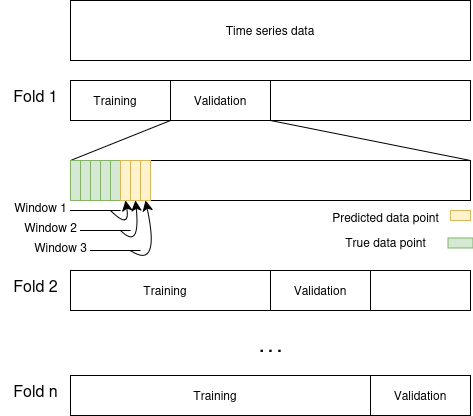
\includegraphics[scale = 0.47]{pictures/recursivecv.drawio.png}
    \caption{The recursive structure of the validation fold. The window of data points that are used 
    to predict the next value are shown. The first window being only true data points, subsequent windows
    increasingly include predicted values until only predicted values are considered. The size of the 
    train fold increases with every fold, while the validation fold remains the same size.}
    \label{fig:recursivecv}
\end{figure}

%Every iteration we validate on the validation fold and save the metrics and an increasing weight. 
%The metrics over the folds are averaged taking into account these weights using the following
%formula:

%$$avg = \frac{\sum_{i=1}^{n}(\text{MSE}_{fold_n} * weight_n)}{\sum_{i=1}^n weight_n}$$

\subsection{Long Short-Term Memory (LSTM)}
We used a Long Short-Term Memory (LSTM) neural network to forecast our time series data, building on 
the architecture and tuning strategy described by Vien et al. \cite{kuen2021machine}. Since we are working 
with a univariate time series, the model was set up to predict future values based solely on past 
observations.

Before training, the library we used standardized the data using z-scores to ensure consistent scaling. We 
then performed a three-dimensional grid search to tune the model, exploring different combinations of the 
number of training epochs, the number of hidden units in the LSTM layer, and the number of lagged time 
steps used as input. This helped us find the setup that worked best for our dataset.

The LSTM architecture itself was straightforward: it included a sequence input layer, one LSTM layer with 
a tunable number of units, a fully connected layer, and an output layer. To evaluate the model, we used 
expanding window cross-validation (also known as forward-chaining), which ensured that the model was 
always tested on future data it hadn’t seen during training — an important detail for time series tasks.
Moreover a dropout option of $0.2$ was selected.

We used mean absolute error (MAE) and mean squared error (MSE) to measure performance across folds. The 
final model was chosen based on the average error, weighted by the size of the training data in each fold.

\subsection{LTSM model parameter intialization}
For efficiency purposes we save time during our initial search for an appropriate number of epochs by 
fixing the number of hidden units to $15$ and lagged time steps to $25$, the result of which can be found in table \ref{tab:epoch_performance}. 
These values are the 'averages'
of the values we will iterate over during the later more extensive grid search. 
After we find the best epoch value we do another grid search over the number of hidden units and lagged
time steps. We use the same method as before, but now we fix the number of epochs to the best value
we found in the previous step. 

\begin{table}[h!]
    \centering
    \begin{tabular}{rcc}
    \hline
    \textbf{Epoch} & \textbf{MSE} & \textbf{MAE} \\
    \hline
    10   & 3135.14 & 44.80 \\
    20   & 2659.23 & 40.03 \\
    50   & 2542.56 & 38.15 \\
    100  & 2432.60 & 38.28 \\
    500  & 2488.35 & 38.28 \\
    1000 & 2436.53 & 37.82 \\
    \hline
    \end{tabular}
    \caption{Model performance (MSE and MAE) across different training epochs during initial search}
    \label{tab:epoch_performance}
\end{table}  

\subsection{Temporal Convolutional Neural Network (TCNN)}\label{methodstcnn}
Additionally, we shortly experiment with a temporal convolutional neural network (TCNN) 
\cite{lea2017temporal}. TCNNs are models that utilize 1-dimensional convolutional layers to capture 
temporal dependencies in data. TCNNs make use of dilated convolutions, where a filter is applied 
over a larger receptive field by skipping over input values. This allows modeling of long-range 
dependencies without an increase in computational complexity.

To find the best hyperparameters for our model, we leverage the Optuna Python library 
\cite{optuna}. Optuna optimizes hyperparameters by iteratively generating parameter configurations 
with a probabilistic model, and observing which configurations minimize the weighted test loss. 
This search was performed over 2000 iterations. 

To accelerate the optimization process, we only train the model for 10 epochs each iteration. We 
utilize a mean square error loss function. We use the Adam optimizer for training. In the TCNN 
architecture, we use the same number of channels for each layer to maintain a consistent feature 
dimension throughout the network. This design choice simplifies the optimization process. Table 
\ref{tab:hyperparameter_search} below illustrates what hyperparameters were found, as well as in 
what ranges the search was conducted. The results of this model are described in the supplementary
section \ref{suppltcnnresults} as the validation on the test data was not done in line with the 
assignment.

\begin{table}[h!]
    \centering
    \begin{tabular}{rccc}
    \hline
    \textbf{Hyperparameter} & \textbf{Range} & \textbf{Step Size} & \textbf{Found Value} \\
    \hline
    \text{number of previous steps} & [10, 60] & 10 & 60 \\
    \text{channels per layer}       & [2, 40]  & 2  & 40 \\
    \text{layers}                   & [2, 5]   & 1  & 2 \\
    \text{kernel size}             & [3, 9]   & 2  & 3 \\
    \text{learning rate}           & [1e-5, 1e-2] & Log Scale & 7.49e-3 \\
    \hline
    \end{tabular}
    \caption{Hyperparameter search ranges, step sizes, and found values.}
    \label{tab:hyperparameter_search}
\end{table}



\section{Results}
\subsection{Grid search}
Doing another grid search using 50 Epochs which we found from our earlier search we group the results by
number of steps looking back 'lags' and number of hidden units. In table \ref{tab:lag_hidden_performance} we can see that
the lowest MSE is at lag = $15.0$ and hidden units = $100$. The lowest MAE is at lag = $35.0$ and hidden units = $50$.

\begin{table}[h!]
    \centering
    \begin{tabular}{r r r r}
    \hline
    \textbf{Lag} & \textbf{Hidden Units} & \textbf{MSE} & \textbf{MAE} \\
    \hline
    5.0  & 5   & 5216.51  & 51.62 \\
      & 10  & 4690.37  & 49.38 \\
      & 20  & 4979.76  & 53.16 \\
      & 50  & 15547.00 & 81.46 \\
      & 100 & 104445.60 & 139.39 \\
    \hline
    15.0  & 5   & 4686.33  & 53.09 \\
      & 10  & 2371759.00 & 477.48 \\
      & 20  & 4746.73  & 52.84 \\
      & 50  & 4764.41  & 57.50 \\
      & 100 & 3581.54  & 49.32 \\
    \hline
    25.0  & 5   & 4031.51  & 50.03 \\
      & 10  & 4458.75  & 49.04 \\
      & 20  & 5126.04  & 49.71 \\
      & 50  & 6044.41  & 56.84 \\
      & 100 & 4737.58  & 49.49 \\
    \hline
    35.0  & 5   & 4963.18  & 51.81 \\
      & 10  & 4913.51  & 48.33 \\
      & 20  & 4654.49  & 46.13 \\
      & 50  & 4955.10  & 45.42 \\
      & 100 & 5091.84  & 46.26 \\
    \hline
    50.0  & 5   & 6657.15  & 63.24 \\
      & 10  & 5439.13  & 50.24 \\
      & 20  & 5220.59  & 47.16 \\
      & 50  & 4836.12  & 46.71 \\
      & 100 & 5222.38  & 47.17 \\
    \hline
    \end{tabular}
    \caption{Model performance (MSE and MAE) for varying lag values and number of hidden units}
    \label{tab:lag_hidden_performance}
\end{table}
    
For our LSTM model with $\textsc{epochs} = 50$, hidden units = $50$ and number of lags = $35$ we 
find the better model achieving a MAE $38.49$ of and a MSE of $2766.98$ on the test data 
(recursively predicted as mentioned in Section \ref{traindataengineer}). A plotting of our 
predicted values against the true values of the provided test data are shown in Figure

\begin{figure}
    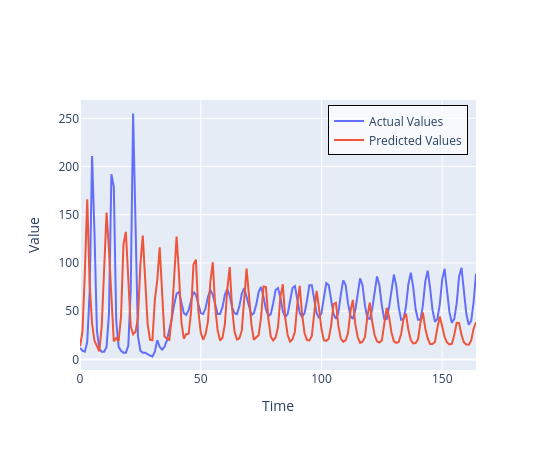
\includegraphics[scale=0.5]{pictures/newmodelresultlag35hu50.png}
    \caption{LTSM predictions vs Actual values. The plotted values are the recursively predicted 
    values by our LTSM model using $50$ epochs, $35$ lags and $50$ hidden units}
    \label{fig:modelresults}
\end{figure}

\section{Discussion}
As described in our methods section we used a recursive approach to predict future values of the 
time series (see Figure \ref{fig:recursivecv}). We did this for the entire validation folds length 
and use this "recursive loss" as a metric to evaluate the model. However it would have been 
interesting to compare this with a non-recursive approach, where we would predict the next value 
using only the true variables instead of the predicted values. That way you can't accumulate faults 
made earlier.  
A limitation in our approach is that we did not use more than one layer whereas using more could be
more beneficial.

\section*{AI statement}
GitHub Copilot was used to assist in writing this report. It was used to generate code snippets and
to help with the writing of the text. Moreover ChatGPT was used to format the single paper source 
as a '$\backslash$bibitem' and the tables in \LaTeX formatting.


\begin{thebibliography}{9}

    \bibitem{kuen2021machine}
    T. Kuen, L. R. F. Rose, W. K. Kong, and B. S. Vien,\\
    \textit{A machine learning approach for anaerobic reactor performance prediction using Long 
    Short-Term Memory Recurrent Neural Network},\\
    Materials Research Proceedings, vol. 18, 2021.\\
    Publisher: Materials Research Forum LLC.

    \bibitem{lea2017temporal}
    C. Lea, M. D. Flynn, R. Vidal, A. Reiter, and G. D. Hager,\\
    \textit{Temporal convolutional networks for action segmentation and detection},\\
    Proceedings of the IEEE Conference on Computer Vision and Pattern Recognition, pp. 156--165, 2017.

    \bibitem{optuna}
    Optuna, \textit{Optuna: A hyperparameter optimization framework}, \url{https://optuna.org}, 2019.
    
\end{thebibliography}

\clearpage
\onecolumn
\section*{Supplementary TCNN results}\label{suppltcnnresults}
The TCNN model achieved a mean absolute error of 28.68 and a mean squared error of 3.26. Using the
found values as described in Table \ref{tab:hyperparameter_search}. It is important to note that in
Figure 

\begin{figure}[H]  % Force the figure to appear exactly here
    \begin{subfigure}{0.45\textwidth}  % Adjust width to fit on the page
        \centering
        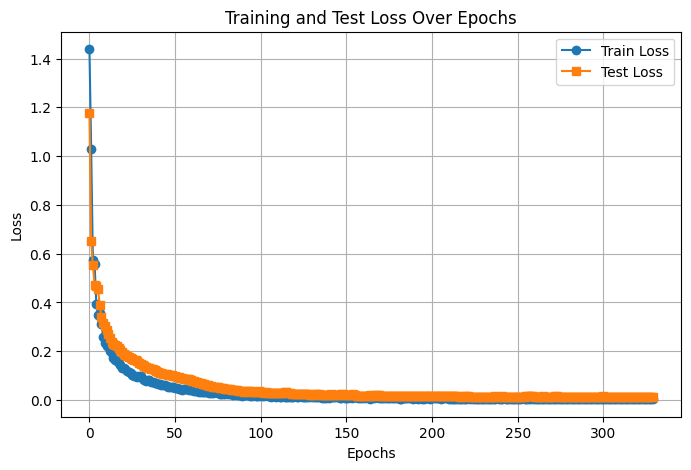
\includegraphics[scale=1]{pictures/train_test_curve.png}
        \caption{Train vs. Test Curve. Here are the results of the loss as described in section 
        \ref{methodstcnn}. It is important to note that these are not recursively predicted values.}
        \label{fig:train_test_curve}
    \end{subfigure}
\end{figure}

\newpage

\begin{figure}[H]        
    \begin{subfigure}{0.45\textwidth}
        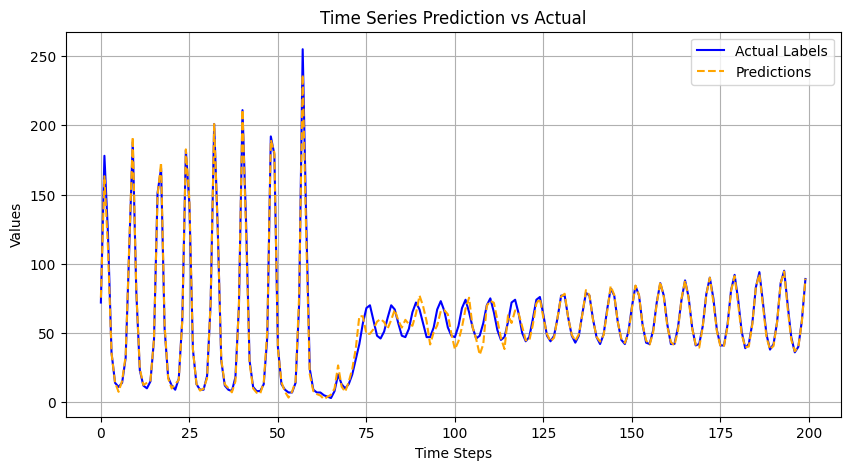
\includegraphics[scale=0.8]{pictures/actual_vs_pred.png}
        \caption{Actual vs. Predicted. The non-recursively predicted values plotted against the
        true test values.}
    \end{subfigure}
    
    \vspace{0.5cm} % Adds a bit of space between the images
    
    \begin{subfigure}{0.45\textwidth}
        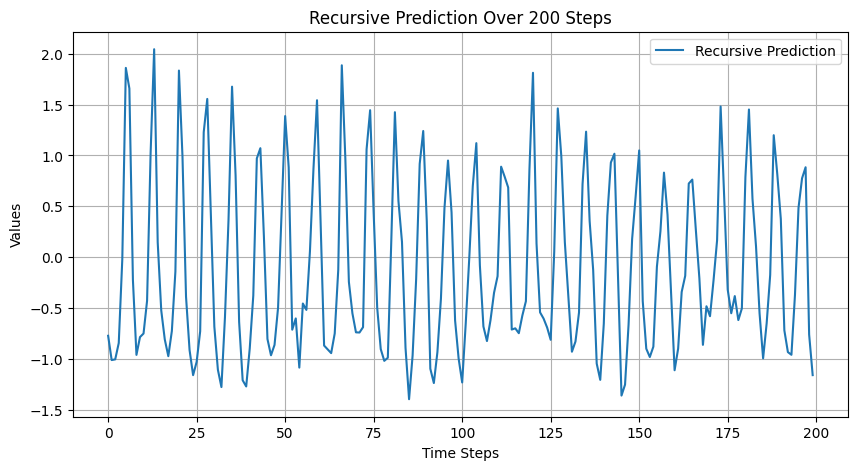
\includegraphics[scale=0.8]{pictures/recursive_predictions.png}
        \caption{Recursive Predictions of the TCNN model. These are the next $200$ recursively
        values as produced by the TCNN model.}
    \end{subfigure}
\end{figure}

\end{document}